% 图 1.5 氢原子中绕核轨道运动的电子
\documentclass[tikz,border=5pt]{standalone}
\usetikzlibrary{arrows.meta}
\usepackage{amsmath}
\usepackage{bm}
\usepackage{fontspec}
\setmainfont{Times New Roman}
\begin{document}
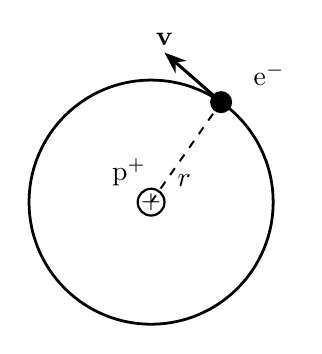
\begin{tikzpicture}[line width=1.0pt,>=Stealth]
% 轨道
\draw (0,0) circle (1.55);
% 质子
\draw[line width=0.8pt,fill=white] (0,0) circle (0.17);
\node at (0,0) {\small$+$};
\node at (-0.28,0.38) {$\mathrm{p}^+$};
% 电子（轨道右上方）
\fill (55:1.55) circle (0.14);
\node at (1.5,1.62) {$\mathrm{e}^-$};
% 速度矢量（切线方向）
\draw[->,line width=1.1pt] (55:1.55) -- ++ (-0.72,0.63)
  node[above,inner sep=2pt] {$\mathbf{v}$};
% 半径 r（虚线）
\draw[dashed,line width=0.7pt] (0,0) -- (55:1.55);
\node at (0.42,0.28) {$r$};
\end{tikzpicture}
\end{document}
